\chapter{Computation Design with Microstructures}
\label{ch3:topopt}
Many engineering problems focus on the design of complex structures that needs to meet high level objectives such as the capability to support localized stresses, optimal tradeoffs between compliance and mass, minimal deformation under thermal changes, etc. One very popular approach to design such structures is topology optimization.
Topology optimization generally refers to discretizing the object of interest into small elements and optimizing the material distribution over these elements in such a way that the functional goals are satisfied \cite{bendsoe2004topology}. Traditionally, topology optimization focused on designs made of homogeneous materials and was concerned with macroscopic changes in the object geometry.
With the advent of multi-material 3D printing techniques, it is now possible to play with materials at a much higher resolution, allowing to obtain much finer designs and, thus, improved functional performances.
Unfortunately, standard techniques for topology optimization do not scale well and they cannot be run on objects with billions of voxels. This is because the number of variables to optimize increases linearly with the number of cells in the object. Since many current 3D printers have a resolution of 600DPI or more, a one billion voxel design occupies only a 1.67 inch cube.

Most previous algorithms working in the material space focused on optimizing a single material property such as density or material stiffness, for which analytical formulas describing the property bounds exist \cite{Allaire93Bounds}. On the contrary, optimizing the structure and material distribution of an object in a high dimensional material property space remains an open problem. In this work, we propose a new computational framework for topology optimization with microstructures that supports design spaces of multiple dimensions. We start by computing the gamut of the material properties of the microstructures by alternating stochastic sampling and continuous optimization. This gives us a {\it discrete} representation of the set of achievable material properties, from which we can construct a {\it continuous} gamut representation using a level set field. We then reformulate the topology optimization problem in the continuous space of material properties and propose an efficient optimization scheme that finds the optimized distributions of multiple material properties simultaneously inside the gamut.
Finally, in order to obtain fabricable designs, we map the optimal material properties back to discrete microstructures from our database.

Our general formulation can be applied to a large variety of problems. We demonstrate its efficacy by designing and optimizing objects in different material spaces using isotropic, cubic and orthotropic materials. We apply our algorithm to various design problems dealing with diverse functional objectives such as minimal compliance and target strain distribution. Furthermore, our approach utilizes the high-resolution of current 3D printers by supporting designs with trillions of voxels. We fabricate several of our designs, thus, demonstrating the practicality of our approach.

The main contributions of our work can be summarized as follows:
\begin{itemize}
	\item We present a fully automatic method for computing the space of material properties achievable by microstructures made of a given set of base materials.
	\item We propose a generic and efficient topology optimization algorithm capable of handling objects with a trillion voxels. The key of our approach is a reformulation of the problem to work directly on continuous variables representing the material properties of microstructures. This allows us to cast topology optimization as a reasonably sized constrained optimization problem that can be efficiently solved with state of the art solvers.
	\item We validate our method on a set of test cases and demonstrate its versatility by applying it to various design problems of practical interest.
\end{itemize}
\section{Overview}
Given as input a set of base materials, an object layout, and functional objectives, the goal of our system is to compute the material distribution inside the object in order to optimize these functional objectives. In our approach, we do not solve the problem directly, instead we work with microstructures made of the base materials and the space of physical material properties spanned by them. The complete pipeline of our system, illustrated in Figure \ref{fig:overview}, can be decomposed into three stages.
\begin{figure}
	\centering
	\includegraphics[width=.95\linewidth]{figs/Overview.pdf}
	\caption{
		Algorithm overview. We start by precomputing the gamut of material properties that can be achieved with all material microstructures of a given size. Next, we run our topology optimization algorithm that optimizes the material properties of the object within this gamut such as to minimize some functional objective. Finally, we map the optimal continuous material properties back to microstructures from our database to generate a printable object.
	}
	\label{fig:overview}
\end{figure}
\paragraph{Material Space Precomputation}
In the first stage, we estimate the gamut of material properties covered by all possible microstructures made by spatial arrangement of base materials. 
Since exhaustively computing the properties of all these microstructures is, in practice, intractable, we progressively increase the material space by alternating a stochastic search and a continuous optimization. The first step introduces discrete changes in the materials of the microstructures and allows emergence of new types of microstructures. The second step allows to locally push the material space boundaries by refining the microstructure shapes. After completing this stage, we obtain a discrete representation of the space of material properties and the mapping between these properties and the corresponding microstructures.

\paragraph{Gamut-based Continuous Topology Optimization}
In the second stage, we construct a smooth continuous gamut representation of the material property space by using a level set field. We define our topology optimization problem directly in this space. Our approach minimizes the objective function over possible material parameters while asking for strict satisfaction of the physics constraints -- typically, the static equilibrium -- as well as the strict satisfaction of the physical parameter bounds. Taking advantage of our gamut representation as a level set, we formulate this last constraint as limiting the material properties to stay on the negative side of the level set. This guarantees that the material properties that we use in the optimization are always physically realizable.

\paragraph{Fabrication-oriented Microstructure Mapping}
In the last stage, we generate a printable result by replacing each cell in the object layout with a microstructure whose material properties are the closest to the continuous material assignment resulting from the optimization. We also take into account the boundary similarity across adjacent cell interfaces to improve the connectivity between microstructures. This results in a complex, high-resolution, multi-material model with optimized functional specifications.

\section{Material Space Exploration}
\label{sec:sampling}

\begin{figure*}[t]
	\centering
	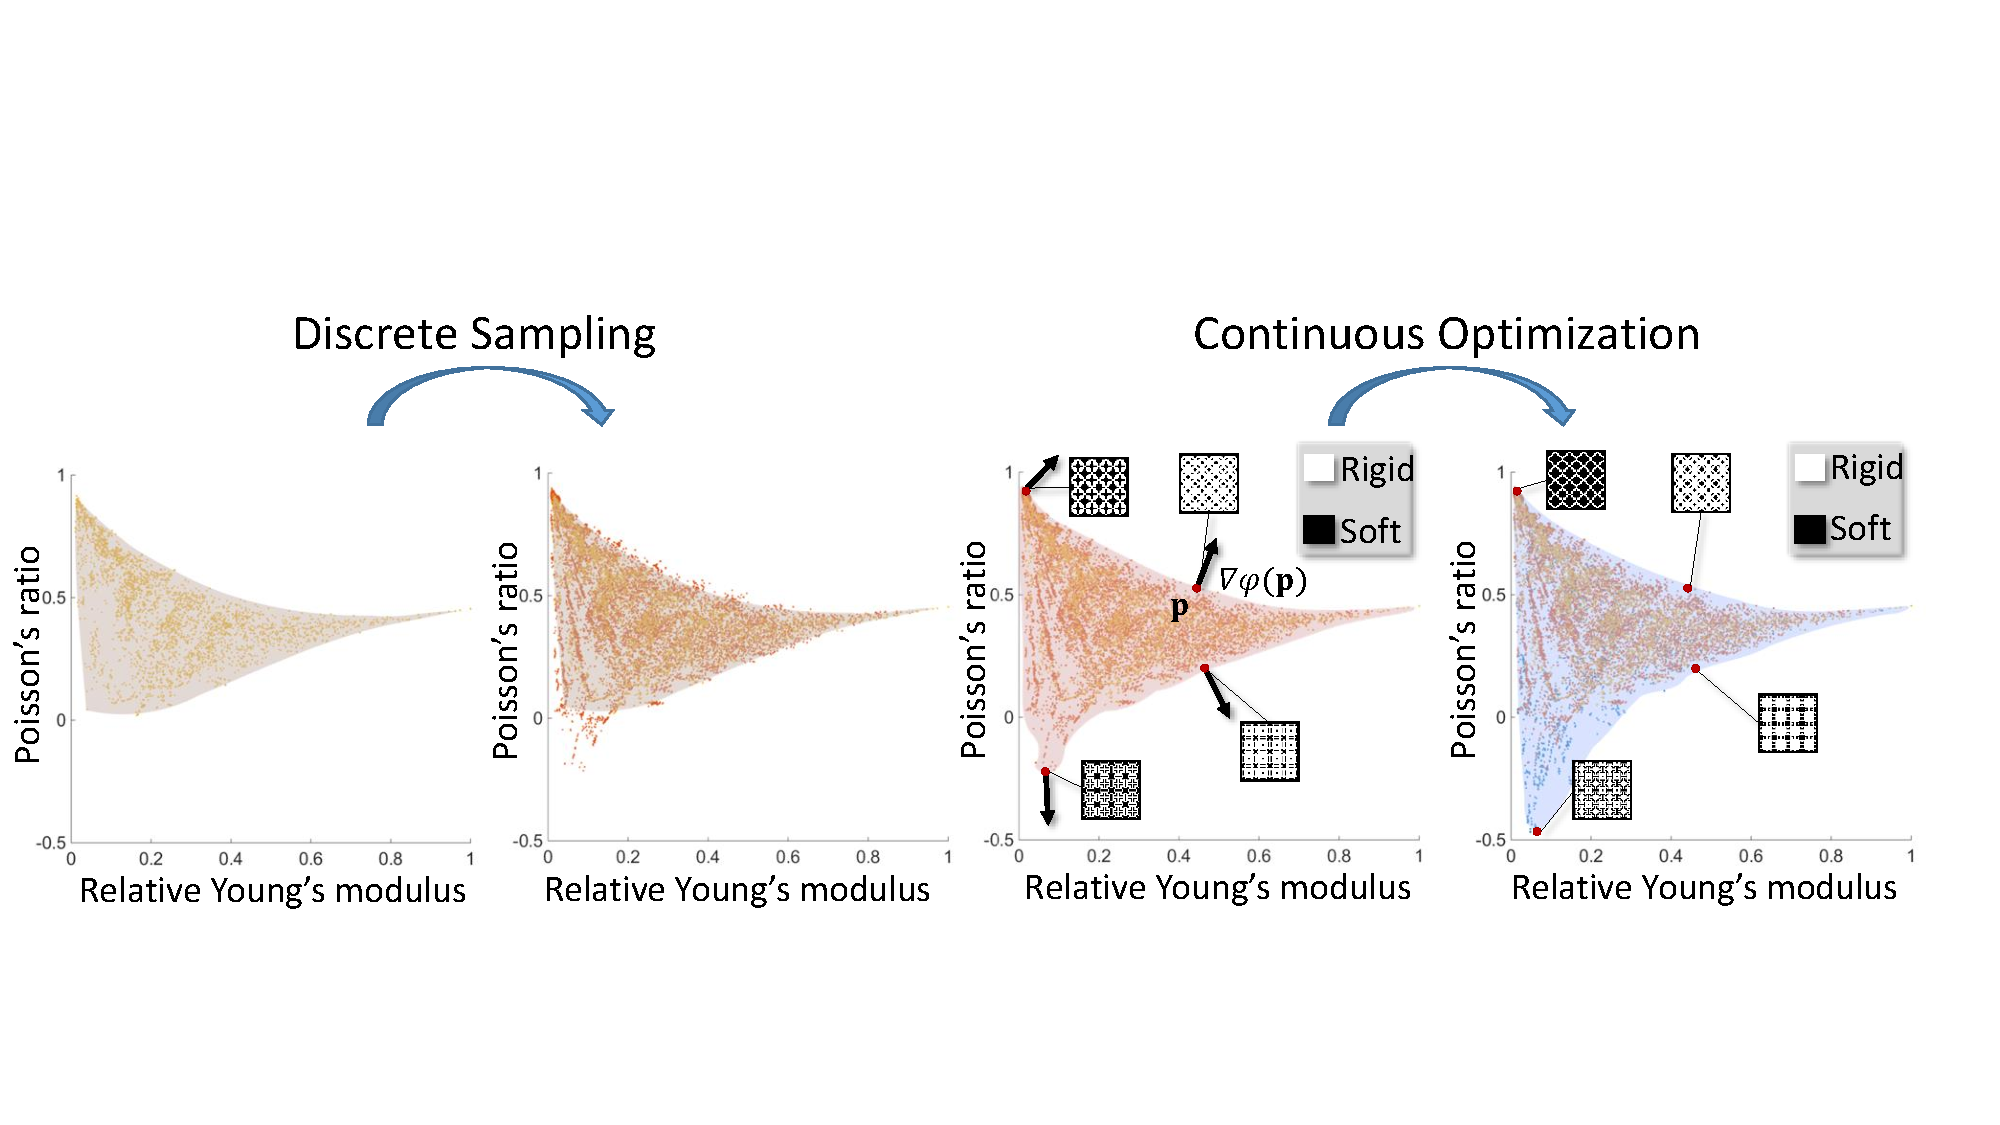
\includegraphics[width=.95\linewidth]{figs/topsampling.pdf}
	\caption{One cycle of computing the microstructure gamut. 
		Given a set of samples, we compute a signed distance function approximating the material gamut (\emph{left}) and randomly perturb microstructures lying near the boundary to provide new seeds to the continuous algorithm (\emph{middle left}). We then update the distance field and use the gradient of the signed distance function at the the boundary to define new target material points (\emph{middle right}). These target material points are used in a continuous optimization that generates new samples (\emph{right}).} 
	\label{fig:lssampling}
\end{figure*}

The first step in our pipeline is to determine the space of physical properties that can be achieved when combining the base materials into microstructures of a predefined size.

Computing the mechanical properties of microstructures, when arranged in periodic tilings, can be performed by probing the structure using a physical simulation. This approach, based on the homogenization theory, is a common practice and has been widely used in the past \cite{Allaire2012,Schumacher:2015,Panetta:2015}. However, while inferring the homogenized properties of individual microstructures is not particularly challenging, analyzing the space covered by {\it all} combinations of base materials is much more difficult due to the combinatorial explosion in the number of possible material arrangements. As an example, $16\times16\times16$ lattices made of only two materials  corresponds to $2^{4096}$ microstructures: exhaustively probing all microstructures is clearly an impossible task.
To address this issue, two possible avenues can be pursued:(i) we can try to sample the space of the microstructures, (ii) we can rely on the continuity between material parameters of the individual voxels and macroscopic properties of the microstructures in order to generate new microstructures with desired properties. This second option is effective in reaching locally optimal values in the material property space. However, the function that maps the material assignment to material properties is nonlinear. In particular, very different microstructures can correspond to the same point in the material property space. Additionally, since the ratio of materials in each cell is bounded between zero and one, the continuous optimization converges slowly or stops moving when material distributions in many cells are at the lower or upper bound. Being able to jump out of a local optimum and discovering different variants is important in order to provide new exploration regions. We leverage these two approaches by combining them in a scheme that alternates between a stochastic search and a continuous optimization. We provide the technical details in the rest of this section.

\subsection{Discrete Sampling of Microstructures}
We aim at sampling the space of material assignments, i.e. microstructures, in such a way that we maximize the number of samples corresponding to microstructures whose material properties lie in the vicinity of the material gamut boundaries. We do not draw all samples at once but progressively enrich the database of microstructures as we refine our estimation of the material gamut boundaries. This sampling strategy is motivated by the observation that a small change in the material assignment of a microstructure generally -- but not always -- translates to a small change of its material properties. By modifying microstructures located near the current boundaries of the material property gamut, we are likely to generate more structures in this area, some of which will lie outside of the current gamut.

Given a population of microstructures to evolve, we generate new samples from each microstructure by changing its material at random voxel locations. To rationalize computational resources, we want to avoid revisiting the same voxel twice. But we do not want to privilege any particular order either. \citet{Ritchie2015SOCM} recently presented a Stochastically-Ordered Sequential Monte Carlo (SOSMC) method that provides a suitable approach.
In SOSMC, a population of particles (here, our microstructures) corresponding to instances of a procedural program (here, the sequential assignment of materials to the voxels of the microstructures) are evolved so as to represent a desired distribution. During this process, the programs are executed in a random order and particles are regularly scored and reallocated in regions of high probability. In our particular settings, we use the scoring function
\begin{equation}
s(\mathbf{p_i}) = \frac{\Phi(\bf p_i)}{D(\bf p_i)} \times \frac{1}{D(\bf p_i)},
\label{eq:score_fct}
\end{equation}
where $\Phi(\bf p_i)$ is the signed distance of the material properties of particle $i$ to the gamut boundary (see Section \ref{sec:ls}) and $D(\bf p_i)$ is the local sampling density at the location $\bf p_i$. We define the sample density as
\begin{equation}
D(\bf p_i)=\sum_{k}\phi_{k}(\bf p_i)\ ,
\end{equation}
where $\phi_{k}(\bf p)=\left(1-\frac{||\bf p-\bf p_{k}||^{2}_{2}}{h^{2}}\right)^{4}$ are locally-supported kernel functions that vanish beyond their support radius $h$, set to a tenth of the size of the lattice used for the continuous representation of the material gamut (see Section \ref{sec:ls}).

The first term in Equation \ref{eq:score_fct} favors microstructures located near the gamut boundary. The normalization by $D$ allows us to be less sensitive to the local microstructures density and to hit any location corresponding to the same level-set value with a more uniform probability. The second product is used to additionally privilege under-sampled areas.

Particles are resampled using systematic resampling scheme \citep{Douc05resamplingSchmes} that is also used to initiate the population of particles. These particles are then evolved by adding and subtracting beams with random sizes. The sampled structures are then cleaned by removing unsupported components and filling enclosed cavities.

\subsection{Continuous Optimization of Microstructures}
The goal of the continuous optimization is to refine the geometry of the microstructures located at the boundary of the gamut in order to further expand the gamut along the normal directions (Figure \ref{fig:contMicro}).
\begin{figure}[h]
	\centering
	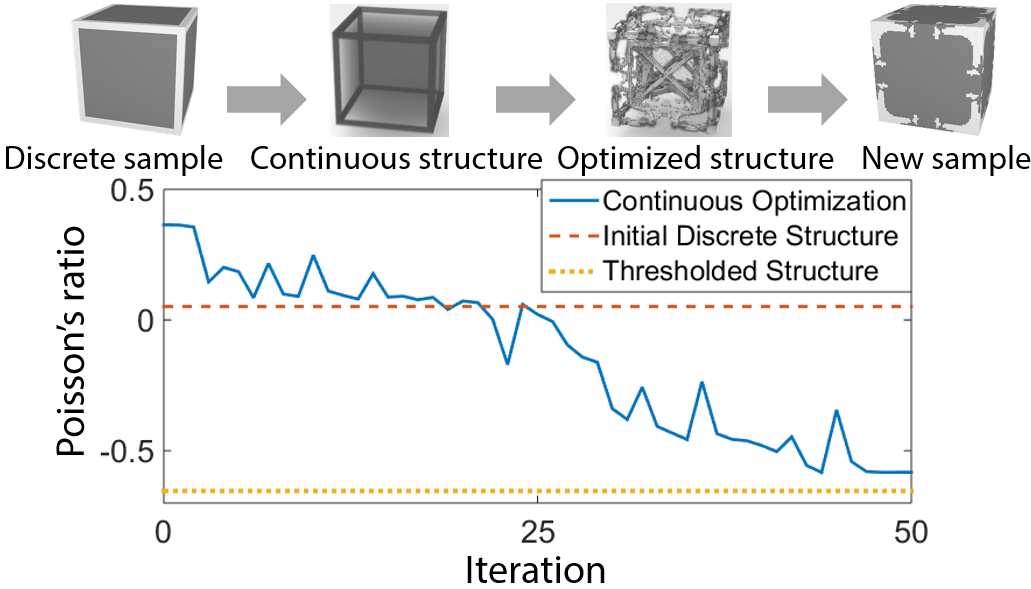
\includegraphics[width=0.9\textwidth]{images/contOpt.png}
	\vspace{-0.2cm}
	\caption{The continuous sampling step uses topology optimization to expand the gamuts by refining existing structures. A good starting point is necessary for the optimization to find better solutions. 
		We use discrete microstructures near the boundary to initialize topology optimization. 
		At convergence, we threshold the values to obtain a new discrete sample.}
	\label{fig:contMicro}
\end{figure}
We start continuous sampling by selecting a subset of microstructures lying on the boundary of the gamut as starting points for the continuous optimization. The discrete structures are mapped to continuous values close to $0.5$. We used $0.5\pm0.3$ in our experiments. Doing so allows the topology optimization algorithms to move freely in the first steps and discover new structures.
We show an example of reducing the Poisson's ratio of an initial structure in Figure \ref{fig:contMicro}. In the plot, the initial Poisson's ratio is close to $0.4$ since the starting point is similar to a homogeneous block.

For each starting structure, we identify target material parameters using the gradient of the level set $\Phi$ at the initial discrete sample point $\bf p$ (see Section \ref{sec:ls}) defined by ${\bf q} = {\bf p} + \nabla \Phi ({\bf p})$. We translate this target material parameters into an elasticity tensor $\bC_0$ and density $\rho_0$. Here $\rho$ is the ratio of the two base materials in the microstructure.

Note that our problem formulation does not restrict us to a particular topology optimization algorithm or material distribution parametrization. We have experimented with two objective functions that worked equally well for our purposes.
The first objective uses an energy based formulation~\cite{xia:2015:design} to compute and optimize the elasticity tensor directly. At a high level, the optimization problem is
\begin{equation}
\arg\min_{\bx} f(\bx) = (\bC(\bx)-\bC_0)^2 + w_{\rho}(\rho-\rho_0)^2, \quad \rho = \sum_{i} x_{i} ,
\end{equation}
where $\bx$ is the ratio of materials in each cell, and $w_{\rho}$ controls the weighting between the displacement term and the density term.
The authors of the method developed parameter heuristics to optimize for difficult cases such as negative Poisson's ratio structures. We naturally arrive at structures with negative Poisson's ratio without the parameter varying step in~\cite{xia:2015:design} since our discrete samples allow us to explore a wide variety of initial designs.

The second objective is formulated using harmonic displacements~\citep{Kharevych2009,Schumacher:2015} $\bG$ instead of the elasticity tensor directly. $\bG$ is a $6\times 6$ symmetric matrix where each row corresponds to a strain in vector form. We use the target elasticity tensor $\bC_0$ to compute the target harmonic displacements matrix $\bG_0$ and minimize the objective function:
\begin{equation}
f(\bx) = (\bG(\bx)-\bG_0)^2 + w_{\rho}(\rho-\rho_0)^2.
\end{equation}
This objective matches soft structures more accurately since entries of $G$ are inversely proportional to material stiffness.

Following the work by \citet{Andreassen2014}, we use the method of moving asymptotes (MMA) \cite{svanberg1987method}) to optimize the objectives using an implementation provided in the NLOPT package \citep{johnson2014nlopt}. We run at most $50$ iterations since it usually converges to a solution within 20-30 steps (Figure~\ref{fig:contMicro}).
MMA makes large jumps during the optimization while keeping track of the current best solution, thus causing the oscillation of the objective value.
To force continuous material ratios towards discrete values, we experimented with the SIMP model with the exponent set to $3$ and the Hashin-Shtrikman bound for isotropic materials
described by~\citet{bendsoe1999material}.

Either interpolation allows us to threshold the final continuous distribution and obtain a similar discrete sample. We tolerate small deviations introduced by the thresholding since our goal is to obtain a microstructure lying outside of the gamut rather than reaching a particular target. In practice, we observed that the material properties of the final discrete structures often did not change significantly after the thresholding step. 

\subsection{Continuous Representation of the Material Gamut }\label{sec:ls}
We represent the gamut of material properties using a signed distance field that is computed from the material points associated to the sampled microstructures.
First, we normalize each coordinate $p_i$ of $\bf p$ to constrain the scope of the level set to an $n$-dimensional unit cube. Then we compute the level set values on the cell centers of an $n$-dimensional Cartesian grid that encloses this unit cube. We draw inspiration from the methods for surface reconstruction used in particle fluid rendering \cite{zhu2005animating,bhatacharya2011level,ando2013highly} and extend it to $n$ dimensions. In this case, a signed distance field is generated from a set of points by evaluating an implicit distance function $\Phi$ at each point $\mathbf{p}\in\mathcal{M}$.
We initialize the signed distance field using the implicit function $\Phi(\mathbf{p})=||\mathbf{p}-\bar{\mathbf{p}}||-r$ from~\citet{zhu2005animating} where $||\cdot||$ is the Euclidean distance between two points in $\mathcal{M}$, and $\bar{\mathbf{p}}$ is the average position of the neighboring points of $\mathbf{p}$ within a range of $2r$. Note that the signed distance is initially defined only near the boundary of the gamut. In order to sample the distance on the entire domain, we propagate the 0-level set surface using the fast marching algorithm and solve an explicit mean curvature flow problem defined as $\partial \Phi / \partial t = \Delta \Phi$~\citep{osher2006level} .

Having a continuous representation of the gamut of materials achievable by the microstructures, we can now reformulate the topology optimization problem directly in the material space.
